\newpage
\section{Architecture Design Patterns}
    There have been different approaches to organize the code base for a rich client side 
    system. In this section, I would like to discuss mainly about two types of architectures
    MVC \cite{mvc} and MVP \cite{mvp}. They are the most relevant design patterns
    for this project as they both separate the presentation layer. 
    In theory the MVP and MVC both are patterns for UI development. It can
    be debated that, there is no UI present at the present moment in this phase of prototyping but
    it can be the case that later on we add some kind of UI functionality i.e. a big button in a
    screen. The view in this module is treated as a dummy where there is no functionality
    available. By doing this there is more freedom in case of possible future changes. 

    \subsection{Model View Controller}
        \label{ssec:mvc}
        This is presumably by far the most used designed pattern adapted by many frameworks like
        \href{https://docs.microsoft.com/en-us/aspnet/core/#build-web-apis-and-web-ui-using-aspnet-core-mvc}
        {Microsoft .NET core MVC}, \href{https://docs.spring.io/spring/docs/current/spring-framework-reference/web.html}
        {Java Spring framework MVC} etc. 

        \begin{figure}[htbp!]
            \centering 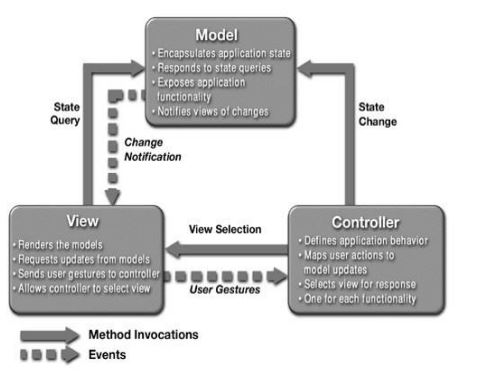
\includegraphics{grafiken/mvc_hotop.jpg}
            \caption{MVC Overview \cite{Hotop2015}}
            \label{fig:mvcOverview}
        \end{figure}

        \par
           The main idea behind is to make a clear separation between domain object and the presentation layer. The two elements should be completely self-
           contained and should be able to work without the presence of the other. This 
           architecture acknowledges three primary aspects. Figure \ref{fig:mvcOverview} 
           gives us an overview of MVC pattern.
           \begin{enumerate}
               \item 
                \textbf{The Model}: This is the layer which represents the data layer. It 
                contains all the relevant data for the business logic. i.e. 
                The route data \ref{code: googleAPi Result} 

               \item 
                \textbf{The View}: This is the user interface where the graphical units area
                placed like buttons, text etc.

               \item 
                \textbf{The Controller} : This layer takes the inputs and changes the two other
                layer accordingly.
           \end{enumerate} 

        

    \subsection{Model View Presenter}
        The MVP architecture is a derivation of the MVC model described in section 
        \ref{ssec:mvc}. The core difference between the MVC and MVP is that the presenter
        tales in the role as the "middle man". This means that the presenter is the only
        entity that talk with the model and view upon request and makes the changes. 
        \cite{Potel}. Figure \ref{fig:mvpOverview} depicts the relationship between the 
        three entities.

        \begin{figure}[htbp!]
            \centering 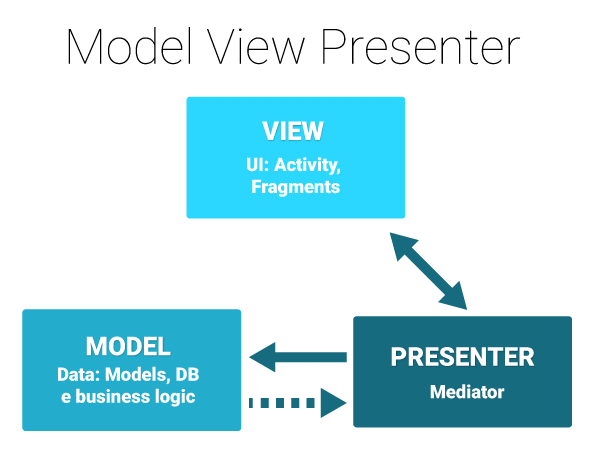
\includegraphics[scale=0.5]{grafiken/mvp.jpg}
            \caption{MVP Overview 
            \href{https://cms-assets.tutsplus.com/uploads/users/1308/posts/26206/image/MVP-Android.png}{refrence}}
            \label{fig:mvpOverview}
        \end{figure}

    \subsection{Evaluation}
        It has been a discussion what is the best design pattern to be used and in the 
        android community MVP is the most favored. There are a couple of reasons why 
        MVP is preferred over MVC because it could be the case that the views would be
        coupled to the interface and the data layers and could get very hard to maintain
        later on. MVP makes the views independent from the data source which makes it
        easier to manage and extend.


